\chapter{Road map}\label{chap:roadmap}

\section{ Road map }
To simplify the problem of moving around the large map, which presumably had to
be done often, the concept of a roadmap was adopted. This, together with cell
division would create  layers of abstraction. When using the road map, no
knowledge of the cells geometry would be needed.
Creation of the road map

The road map does need to be created based on the the information about the
cells. The cells was represented by pointers to the edges it consisted of. These
edges was in turn made up of pointers, here to vertices, two each. The edges
also contained information on which cells they were part of. There are two
different kinds of edges. Those made out of obstacles, called hard edges and
those that made up boundaries between two cells, called soft edges. The road map
is build up of nodes representing cells and soft edges, because soft edges are
the entrances to the cells. As long as the cells are convex there is a straight
line from every point in the cell to any other. Travelling along the road then
simplifies to a list of straight lines from the soft edges of cells plus the
small distances to get on and off the roadmap from a point within the cell.

The actual road map was created by creating two lists of nodes, one of cell
nodes and one of soft edge nodes. Then when all nodes exist, their
interconnectivity is saved as information in every node, by the other nodes it
immediately connects to, altogether creating a graph. This is done by running
through the cells belonging to a soft edge node, and in those cells, running
throug all the soft edges to connect to them. This is done by comparing the the
list of all soft edge nodes to create the right pointers. This gives O(n²) since
the number of edges per cell an the number of cells per soft edge is very small,
but the number of edges in general is large, and this has to be run through
twice. But it was not a big deal, since the creation of the map could be done
offline, since the buildings on the map was considered not to change position,
so the time to execute the creation of the map was not crucial. The picture
below is a visualizaition of the connections between soft edges, the connections
shown in bright white.
Using the road map

The roadmap is used to find a route from one cell to another. The shortest route
is found using BFS by maintaining a sorted list off all possible routes from the
start, shortest route first. The list is expanded one node at a time by adding
the closest node to the shortest route on the list. If a node has already been
visited in the particular search, it cannot be added to a route, because another
route have obviously gotten there earlier and thereby more efficiently. This is
iterated until the soft edge node is reached which is a part of the destination
cell. The route that reaches this node must be the shortest since only the
shortest route is expanded every iteration. In the figure below is a
visualization of a rout from the first cell in the upper left corner to another
cell.

\begin{figure}[htb] \centering 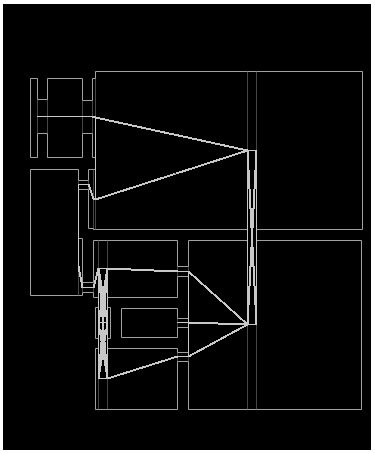
\includegraphics[width=\textwidth,trim=0 0 0
0]{graphics/pic1.png}
	% trim=l b r t (can cut off from every side)
	\caption{Choosing overall coverage plan}
	\label{fig:Choosingoverallcoverageplan}			
\end{figure}


The road map was also used to choose the order in which the cells should be
visited. Here a DFS was chosen so to only travel a short distance between cells
every time, though some long distance travelling was bound to happen also. Given
a starting point, a list of cell nodes to visit was created by recursively visit
every cell node, marking it as visited when entering it, and marking it as
having all childs explored when returning from the recursive function of that
cell.

\begin{figure}[htb] \centering 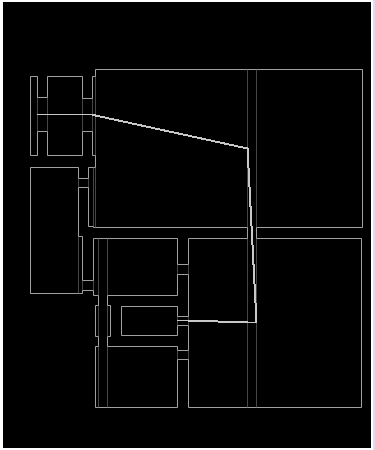
\includegraphics[width=\textwidth,trim=0 0 0
0]{graphics/pic2.png}
	% trim=l b r t (can cut off from every side)
	\caption{Road map results}
	\label{fig:Roadmapresults}			
\end{figure}


A simulation of finding a route from every cell to the next in the overall
coverage plan and summing up the length resulted in a total traveling length for
moving between cells of 8849.96 meters.



